\documentclass[a4paper, 10pt, fleqn]{article}
\usepackage[utf8]{inputenc}
\usepackage[czech]{babel}
\usepackage{graphicx}
\usepackage{geometry}
 \geometry{
 a4paper,
 total={170mm,257mm},
 left=20mm,
 top=20mm,
 }
\usepackage{amsmath}
\begin{document}
\begin{center}

\includegraphics[scale=0.15]{IEL_OBR/fit.png}
\\[2.5in]
\LARGE
Elektronika pro informační technologie\\*
2015/2016	
\\*[4.5in]
\end{center}
\LARGE
Jméno: Matějka Jiří \\*
Login: xmatej52 \\*
ID: 187182

\newpage
\section*{Příklad 1}
\subsection*{Zadání}

Stanovte napětí $U_{R3}$ a proud $I_{R3}$\\
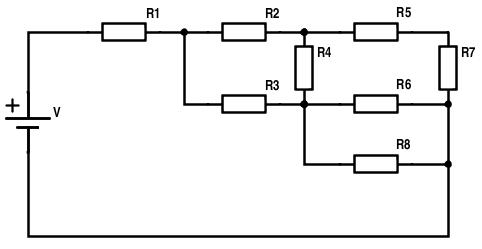
\includegraphics[scale=0.8]{IEL_OBR/1a.png}  \\
\begin{align*}
 R_{1} &= 650 \Omega \\
 R_{2} &= 730 \Omega \\
 R_{3} &= 340 \Omega \\
 R_{4} &= 330 \Omega \\
 R_{5} &= 410 \Omega \\
 R_{6} &= 830 \Omega \\
 R_{7} &= 340 \Omega \\
 R_{8} &= 220 \Omega \\
 U &= 95 V \\
\end{align*}
\subsection*{Řešení příkladu}
 Použijeme metodu postupného zjednodušování obvodu \\
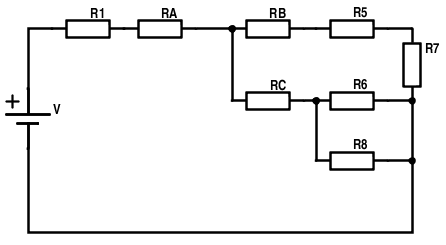
\includegraphics[scale=0.8]{IEL_OBR/1b.png} \\*
\begin{align*}
 R_{A} &= \frac{R_{2} \times R_{3}}{R_{2} + R_{3} + R_{4}} \\
 R_{B} &= \frac{R_{2} \times R_{4}}{R_{2} + R_{3} + R_{4}} \\
 R_{C} &= \frac{R_{3} \times R_{4}}{R_{2} + R_{3} + R_{4}} \\
\end{align*}
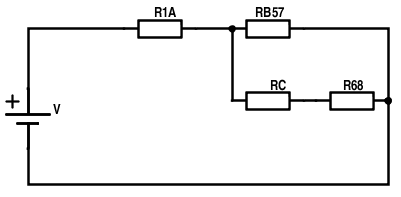
\includegraphics[scale=0.8]{IEL_OBR/1c.png}\\*
\begin{align*}
 R_{1A} &= R_{1} + R_{A} \\*
 R_{68} &= \frac{R_{6} \times R_{8}}{R_{6} + R_{8}} \\*
 R_{B57} &= R_{B} + R_{5} + R_{7} \\
\end{align*}
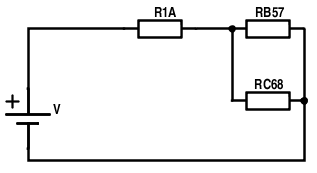
\includegraphics[scale=1]{IEL_OBR/1d.png}\\*
 $R_{C68} = R_{C} + R_{68}$ \\
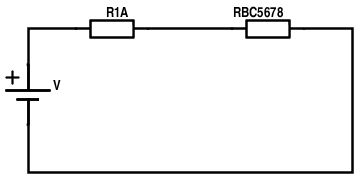
\includegraphics[scale=1]{IEL_OBR/1e.png}\\*
 $R_{BC5678} = \frac{R_{B57} \times R_{C68}}{R_{B57} + R_{C68}}$ \\
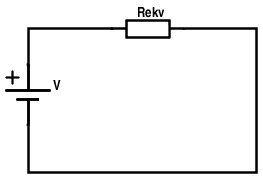
\includegraphics[scale=1]{IEL_OBR/1f.png}\\*
 $R_{ekv} = R_{1A} + R_{BC5678}$ \\
 Nyní můžeme vypočítat proud $I$ \\*
 $I = \frac{U}{R_{ekv}}$ \\
 Když známe celkový proud v obvodu, budeme postupně opět počítat napětí a proud
 na jednotlivých rezistorech. \\*
\begin{align*}
 U_{1A} &= I \times R_{1A} \\
 U_{1} &= I \times R_{1} \\
 U_{A} &= I \times R_{A} \\
 U_{BC5678} &= I \times R_{BC5678} \\
 I_{B57} &= \frac{U_{BC5678}}{R_{B57}} \\
 I_{C68} &= \frac{U_{BC5678}}{R_{C68}} \\
 U_{C} &= I_{C68} \times R_{C} \\
 U_{68} &= I_{C68} \times R_{68} \\
 U_{B} &= I_{B57} \times R_{B} \\
 U_{5} &= I_{B57} \times R_{5} \\
 U_{7} &= I_{B57} \times R_{7} \\
 I_{6} &= \frac{U_{68}}{R_{6}} \\
 I_{8} &= \frac{U_{68}}{R_{8}} \\
\end{align*}
 Nyní použijeme Kirchhoffovy zákony pro výpočet zbylých napětí \\*
\begin{align*}
 0 &= U_{1} + U_{3} + U_{68} - U \\
 U_{3} &= U - U_{1} - U_{68} \\
 0 &= U_{1} + U_{2} + U_{5} + U_{7} - U \\
 U_{2} &= U - U_{1} - U{5} - U{7} \\
 0 &= U_{2} + U_{4} - U_{3} \\
 U_{4} &= U_{3} - U_{2} \\
\end{align*}
 A Ohmovy zákony pro výpočet proudů na rezistorech $R_{2}, R_{3}$ a $R_{4}$ \\*
\begin{align*}
 I_{2} &= \frac{U_{2}}{R_{2}} \\
 I_{3} &= \frac{U_{3}}{R_{3}} \\
 I_{4} &= \frac{U_{4}}{R_{4}} \\
\end{align*}
Po dosazení číselných hodnot zjistíme, že $U_{3}$, repsektive $U_{R3} = 22.2525 V$ a
$I_{3}$, respektive $I_{R3} = 0.0654 A$.
\newpage
\section*{Příklad 2}
\subsection*{Zadání}
Stanovte napětí $U_{R3}$ a proud $I_{R3}$. Požijte metodu Théveninovy věty. \\*
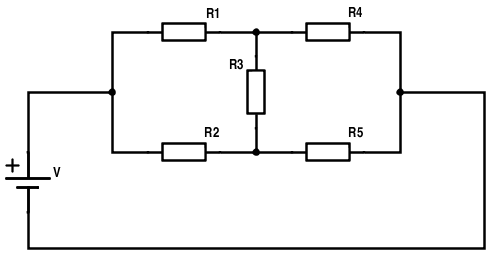
\includegraphics[scale=0.8]{IEL_OBR/2a.png} \\*
\begin{align*}
 U &= 250 V \\
 R_{1} &= 335 \Omega \\
 R_{2} &= 625 \Omega \\
 R_{3} &= 245 \Omega \\
 R_{4} &= 600 \Omega \\
 R_{5} &= 180 \Omega \\
\end{align*}
\newpage
\subsection*{Řešení příkladu}
Odpojíme zátěž $R_{3}$. \\*
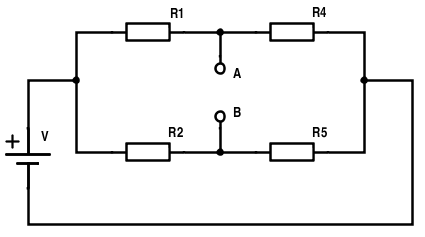
\includegraphics[scale=0.8]{IEL_OBR/2c.png} \\*
A pokusíme se zbylou část obvodu "přeměnit"~na ideální zdroj napětí: \\*
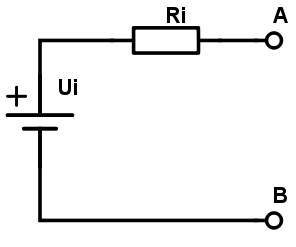
\includegraphics[scale=0.5]{IEL_OBR/2d.png} \\*
Zjistime Ui: \\
\begin{align*}
 U_{i} &= U_{R2} - U_{R1} \\
 U_{R1} &= U \times \frac{R_{1}}{R_{1} + R_{4}} \\
 U_{R2} &= U \times \frac{R_{2}}{R_{2} + R_{5}} \\
\end{align*}
\newpage
\noindent
Nyní spočítáme vnitřní odpor ideálního zdroje ($R_{i}$) pomocí kterého následně
určíme $I_{R3}$. Díky Ohmova zákonu poté budeme schopni dopočítat $U_{R3}$. \\*
\begin{align*}
 R_{i} &= \frac{R_{2} \times R_{5}}{R_{2} + R_{5}} + \frac{R_{1} \times R_{4}}{R_{5} + R_{4}0}\\
 I_{R3} &= \frac{U_{i}}{R_{i} + R_{3}} \\
 U_{R3} &= I_{R3} \times R_{3} \\
\end{align*}
Po dosazení číselných hodnot zjistíme, že $U_{3}$, repsektive $U_{R3} = 39.8621 V$ a
$I_{3}$, respektive $I_{R3} = 0.1627 A$. 

\newpage
\section*{Příklad 3}
\subsection*{Zadání}
Stanovte napětí $U_{R3}$ a proud $I_{R3}$. Použijte metodu uzlových napětí
($U_{A}, U_{B}, U_{C}$).\\*
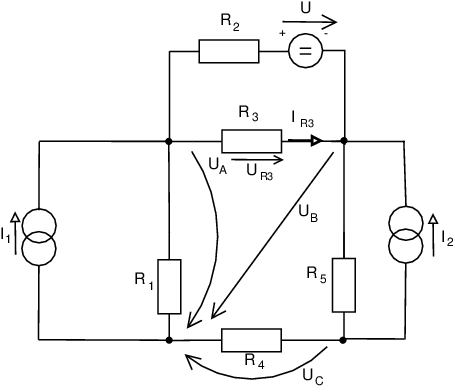
\includegraphics[scale=0.5]{IEL_OBR/3a.png} \\*
\begin{align*}
 U &= 145 V \\
 I_{1} &= 0.75 A \\
 I_{2} &= 0.85 A \\
 R_{1} &= 480 \Omega \\
 R_{2} &= 440 \Omega \\
 R_{3} &= 530 \Omega \\
 R_{4} &= 360 \Omega \\
 R_{5} &= 225 \Omega \\
\end{align*}

\subsection*{Řešení příkladu}
Sestavíme rovnice proudů v uzlech:\\*
\begin{align*}
A&: I_{1} + I_{R2} - I_{R1} - I_{R3} &= 0 \\
B&: I_{R3} + I_{2} - I_{R2} - I_{R5} &= 0 \\
C&: I_{R5} - I_{R4} - I_{2} &=0 \\
\end{align*}
A podle Kirchhoffových a Ohmových zákonů sestavíme rovnice:\\
\begin{align*}
&R_{1} \times I_{R1} - U_{a} &= 0\\
&R_{2} \times I_{R2} - U - U_{B} - U_{A} &= 0 \\
&R_{3} \times I_{R3} + U_{B} - U_{A} &= 0 \\
&R_{4} \times I_{R4} - U_{C} &= 0 \\
&R_{5} \times I_{R5} + U_{C} - U_{B} &= 0 \\
\end{align*}
A vyjádříme proudy:
\begin{align*}
I_{R1} &= \frac{U_{A}}{R_{1}}\\
I_{R2} &= \frac{U + U_{B} - U_{A}}{R_{2}} \\
I_{R3} &= \frac{U_{A} - U_{B}}{R_{3}}\\
I_{R4} &= \frac{U_{C}}{R_{4}}\\
I_{R5} &= \frac{U_{B} - U_{C}}{R_{5}}\\
\end{align*}
Proudy dosadíme do rovnic A, B a C. Vypočítáme $U_{A}, U_{B}$ a dosadíme do
$I_{R3} = \frac{U_{A} - U_{B}}{R_{3}}$. Vyjde nám, že $I_{R3} = 0.1806 A$.
Dosadíme do $U_{R3} = R_{3} \times I_{R3}$ a vyjde nám, že $U_{R3} = 95.7140 V$.
\newpage
\section*{Příklad 4}
\subsection*{Zadání}
Pro napájecí napětí platí: $u_{1} = U_{1} \times \sin(\omega t),$
$u_{2} = U_{2} \times \sin(\omega t)$. \\
Ve vztahu pro napětí $u_{C_{2}} =U_{C2} \times \sin (\omega t + \varphi_{C_{2}})$.
Použijte metodu smyčkových proudů.\\[0.8cm]
Pozn: Pomocné směry šipek napájecích zdrojů platí pro speciální okamžik
($t = \frac{\pi}{2\omega}$)."\\
% \newpage
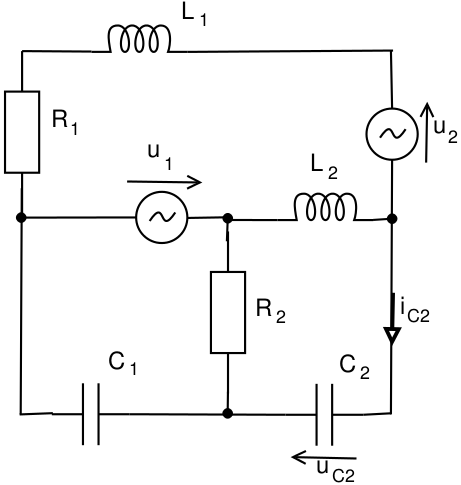
\includegraphics[scale=0.5]{IEL_OBR/4.png}\\*
\begin{align*}
 U_{1} &= 25 V \\
 U_{2} &= 40 V \\
 R_{1} &= 115 \Omega \\
 R_{2} &= 150 \Omega \\
 L_{1} &= 0.1 H \\
 L_{2} &= 0.085 H\\
 C_{1} &= 2.2 \times 10^{-4} F \\
 C_{2} &= 0.95 \times 10^{-4} F \\
 f &= 80 Hz \\
\end{align*}
\newpage
\subsection*{Řešení příkladu}
Přizpůsobíme si obvod pro výpočty:
\begin{align*}
X_{L1} &= \omega \times L_{1} \times j \\
X_{L2} &= \omega \times L_{1} \times j \\
X_{C1} &= \frac{1}{\omega \times C_{1} \times j} \\
X_{C2} &= \frac{1}{\omega \times C_{2} \times j} \\
Z_{1} &= X_{L1} + R_{1} \\
\end{align*}
A sestavíme rovnice:
\begin{align*}
&I_{b} \times Z_{1} - u_{2} + (I_{b} - I_{c}) \times X_{L2} - u_{1} &= 0 \\
&I_{c} \times X_{C2} + (I_{c} - I_{a}) \times R_{2} + (I_{c} - I_{b}) \times X_{L2} &= 0 \\
&u_{1} + (I_{a} - I{c}) \times R_{2} + I_{a} \times X_{C1} &= 0 \\
\end{align*}
Po dosazení hodnot nám vyjde, že:
\begin{align*}
I_{a} &= -2.81292+1.3 \times j \\
I_{b} &= 0.122034 - 0.359255 \times j \\
I_{c} &= -2.46475 + 1.6928 \times j \\
\end{align*}
Výpočet $u_{C2}$:
\begin{align*}
U_{C2} &= X_{C2} \times I_{c} = 35.4500+51.6150 \times j \\
|U_{CV}| &= 62.6164 V \\
\varphi &= \arctan  (\frac{U_{C2}(IM)}{U_{C2}(RE)}) = 0.9690 \\
% u_{c2} &= 62.6164 \times \sin (\omega t + 0.9690) \\
% u_{c2} &= 62.6164 \times \sin (2 \pi f t + 0.9690) \\
% u_{c2} &= 62.6164 \times \sin (160 \pi t + 0.9690) \\
\end{align*}
\newpage
\section*{Příklad 5}
\subsection*{Zadání}
Sestavte diferenciální rovnici popisující chování obvodu na obrázku, dále
ji upravte dosazením hodnot parametrů. Vypočítejte abakytické řešení $u_{c}~=~f(t)$.
Proveďte kontrolu výpočtu dosazením sestavené diferenciální rovnice.\\*
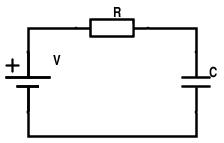
\includegraphics[scale=0.8]{IEL_OBR/5.png}\\*
\begin{align*}
 U &= 12 V \\
 C &= 30 F \\
 R &= 45 \Omega \\
 u_{c}(0) &= 5V \\
\end{align*}
\newpage
\subsection*{Řešení příkladu}
Řešním příkladu je časový průběh: $\frac{du_{c}}{dt}$ \\*
Dále víme, že $I_{c} = I$ a ${u_{c}'} = \frac{1}{C} \times I_{c}$ \\*
Pomoci Kirchhoffových a Ohmových zákonů sestavíme rovnici: \\*
\begin{align*}
 U_{R} + U_{C} - U &= 0 \\
 R \times I + U_{C} - U &= 0 \\
 I &= \frac{U - U_{C}}{R} \\
\end{align*}
Nyní použijeme vztah ${u_{c}'} = \frac{1}{C} \times I_{c}$: \\*
\begin{align*}
 {u_{c}'} &= \frac{1}{C} \times \frac{U - U_{c}}{R} \\
 {u_{c}'} &= \frac{1}{30} \times \frac{12 - U_{c}}{R} \\
 {u_{c}'} &= \frac{12 - U_{C}}{1350} \\
 12 &= 1350 \times {u_{c}'} + U_{C}
\end{align*}
Nyní můžeme spočítat charakteristickou rovnici: \\*
\begin{align*}
 0 &= 1350\lambda + 1 \\
 \lambda &= -\frac{1}{1350} \\
\end{align*}
A díky charakteristické rovnice můžeme sestavit očekávaný tvar řešení:\\*
\begin{align*}
 U_{C} &=c(t) \times e^{\lambda t} \\
\end{align*}
Dosadme hodnoty a zderivujeme: \\*
\begin{align*}
 U_{C} &=c(t) \times e^{-\frac{t}{1350}} \\
 {u_{c}'} &= {c'(t)} \times e^{-\frac{t}{1350}} - \frac{c(t) \times e^{-\frac{t}{1350}}}{1350} \\
\end{align*}
Dosadíne do rovnice $12 = 1350 \times {u_{c}'} + U_{C}$: \\*
\begin{align*}
 {c'(t)} \times e^{-\frac{t}{1350}} - \frac{c(t) \times e^{-\frac{t}{1350}}}{1350} &= \frac{12}{1350} - \frac{c(t) \times e^{-\frac{t}{1350}}}{1350} \\
 {c'(t)} \times e^{-\frac{t}{1350}} &= \frac{12}{1350} \\
 {c'(t)} &= \frac{6 \times e^{\frac{t}{1350}}}{675} \\
\end{align*}
Nyní můžeme začít integrovat: \\
\begin{align*}
 \int{c'(t)}dt &= \int\frac{6 \times e^{\frac{t}{1350}}}{675} dt \\
 c(t) + k &= \frac{6}{675} \times \int e^{\frac{t}{1350}} \\
 c(t) + k &= \frac{6}{675} \times (1350) \times e^{\frac{t}{1350}} \\
 c(t) &= 12 \times e^{\frac{t}{1350}} - k \\
\end{align*}
Dosadíme do rovnice: $u_{c}(t) = c(t) \times e^{-\frac{t}{1350}}$ \\
\begin{align*}
 u_{c}(t) &= (12 \times e^{\frac{t}{1350}} - k ) \times e^{-\frac{t}{1350}} \\
 u_{c}(t) &= 12  - k \times e^{-\frac{t}{1350}} \\
\end{align*}
Počáteční podmíny:
\begin{align*}
 u_{c}(0) &= 12  - k \times e^{-\frac{0}{1350}} \\
 5 &= 12  - k \\
 k &= 7 \\
\end{align*}
Výsledek tedy je $u_{c}(t) = 12  - 7 \times e^{-\frac{t}{1350}}$
\newpage
\section*{Přehled výsledků}
\begin{center}
  \begin{tabular}{ | c | c | c |}
    \hline
    Číslo příkladu & Zadání & Výsledek \\ \hline
    1 & B & U$_{R3} = 22.2525~$V,  I$_{R3} = 0.0654~$A \\ \hline
    2 & E & U$_{R3} = 39.8621~$V, I$_{R3} = 0.1627~$A \\ \hline
    3 & F & U$_{R3} = 95.7140~$V, I$_{R3} = 0.0.1806~$A \\ \hline
    4 & B & $|$U$_{C2}| = 62.6164~$V, $\varphi = 0.9690$\\ \hline
    5 & E & u$_{c}(t) = 12 - 7 \times e^{-\frac{t}{1350}}$ \\ \hline
  \end{tabular}
\end{center}
\end{document}
